\documentclass{article}

\usepackage{french}
 
\pagestyle{headings}
\markright{28/6/1995 \hfill Conservatoire National des Arts et
M\'etiers -- Paris \hfill\ } 

\baselineskip 6pt
\parskip 6pt
\onecolumn
\textwidth 16cm
\textheight 24cm
\hoffset=-2cm
\voffset=-2.5cm
\setlength{\parindent}{0.0cm}
\unitlength 1cm
\input{psfig}
\newtheorem{defin}{D\'efinition}[section]
\newtheorem{exampl}{Exemple}[section]
\def\picwidth{16cm}

\begin{document}
\psfig{figure=dept.epsi} 
\begin{center}
\Large\bf Processus d'Informatisation et Bases de Donn\'ees A \\ 
    Partiel Bases de Donn\'ees\\
\large\bf Mercredi 3 mars 1999
\end{center}

%%%%%%%%%%%%%%%%%%%%%%%%%%%%%%%%%%%%%%%%%%%%%%%%%%%%%%%%%%%%

\vspace*{2cm}

\hrule

Soit $P$ la note du partiel, et $E$ la note
de l'examen final. Alors vous \^etes re\c{c}us si
$E > 7$ ET $Max (E, (E+P)/2) \ge 10$. Donc le partiel vous
permet de r\'ecup\'erer des points sous r\'eserve
d'avoir au moins
7 \`a l'examen final.

\smallskip

\hrule

\vspace*{2cm}

Une station de ski d\'esire cr\'eer une base de donn\'ees
afin d'\'etudier le comportement des touristes. On
s'int\'eresse notamment aux logements occup\'es
dans les h\^otels
et aux pistes fr\'equent\'ees par les skieurs.
La soci\'et\'e RGX-Consulting a \'etabli le
mod\`ele E/A de la figure~\ref{ski}. 
A vous de jouer pour la mise-en-oeuvre de la 
base de donn\'ees.

  \begin{figure}[htb]  
    \centerline{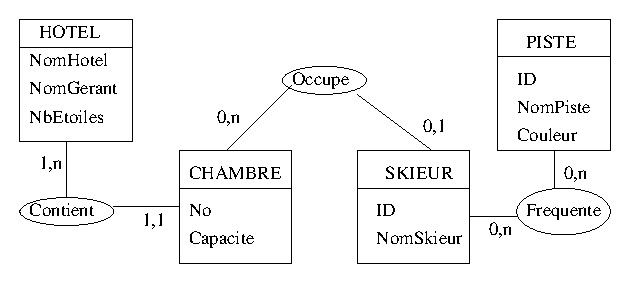
\psfig{width=12cm,figure=partiel99.eps}}  
    \caption{Station de ski}  
    \label{ski}  
  \end{figure}  

\smallskip
{\bf Cr\'eation du sch\'ema}

\begin{enumerate}
   \item ({\bf 5 pts}) Donnez les commandes {\tt CREATE TABLE} d\'ecrivant
         le sch\'ema de la base. Indiquez soigneusement
         les cl\'es \'etrang\`eres et les cl\'es primaires.

         Pour chaque cl\'e \'etrang\`ere, donnez la
        commande {\tt ON DELETE} associ\'ee, en choisissant
        l'option ({\tt SET NULL} ou {\tt CASCADE})
        coh\'erente avec le sch\'ema E/A.

   \item ({\bf 4 pts})
       Pour chacune des contraintes ci-dessous, indiquez
        quelle est la commande SQL2 qu'il faudrait ajouter
        aux cr\'eations de tables. Donnez la syntaxe pr\'ecise,
       ainsi que la table sur
    laquelle porte la contrainte.

   \begin{enumerate}
       \item Les informations suivantes doivent \^etre
        toujours connues\,: la capacit\'e 
          de la chambre, le nom des skieurs
          et la couleur de la piste.
   
       \item Il ne peut pas y avoir deux h\^otels avec le 
             m\^eme g\'erant.
      
       \item La couleur d'une piste est 'verte', 'bleue', 
                'rouge' ou 'noire'.

       \item Le nombre de skieurs dans une chambre ne peut
                 pas d\'epasser la capacit\'e de la chambre.       
   \end{enumerate}
\end{enumerate}
    

\smallskip
{\bf D\'ependances fonctionnelles (3 pts)}


\begin{enumerate}
   \item La d\'ependance fonctionnelle $Skieur \to Hotel$ 
       est-elle v\'erifi\'ee sur le sch\'ema pr\'ec\'edent\,?

    \item Deux chambres peuvent-elles avoir la m\^eme capacit\'e\,?

    \item Un skieur peut-il fr\'equenter deux pistes de couleurs
           diff\'erentes\,?
\end{enumerate}


\smallskip
{\bf Requ\^etes ({\bf 6 pts})}

Sur le sch\'ema obtenu pr\'ec\'edemment, exprimez
en alg\`ebre relationnelle et en SQL les requ\^etes suivantes:

\begin{enumerate}
  \item Liste des noms des pistes rouges.

  \item Nom des h\^otels ayant au moins une chambre de 6 personnes.
        Attention\,: il ne doit pas y avoir de doublon.

  \item Liste des skieurs avec le nom des pistes qu'ils fr\'equentent.

  \item Nom des skieurs log\'es \`a l'h\^otel g\'er\'e
        par Mr Logeais.

  \item Nom des skieurs qui ne fr\'equentent pas de piste.

  \item  Nom des pistes noires fr\'quent\'ees par les clients
        de l'h\^otel g\'er\'e par Mr Toirac.
\end{enumerate}

\smallskip
{\bf Requ\^etes SQL ({\bf 4 pts})}
 
La table suivante contient diverses informations sur
les animaux d'un zoo.

\begin{center} 
{\tt   ANIMAL (idAnimal,Nom, Ann\'ee\_naissance, Esp\`ece, Emplacement)}
\end{center}

R\'epondre aux requ\^etes suivantes
en langage SQL:

\begin{enumerate}
  
  \item Nom des animaux dont l'esp\`ece est indiqu\'ee
       dans la base\,?

  \item Combien d'animaux sur l'emplacement 35\,?

  \item Couples d'animaux (leur nom) occupant le m\^eme emplacement.

   \item Liste des emplacements ayant au moins 4 animaux
     (donner aussi le nombre d'animaux sur l'emplacement).
\end{enumerate}

\begin{center}

\framebox(10,2){{\bf Solution sur le WEB, et au secr\'etariat}}
\end{center}
\end{document}